
\documentclass[tikz]{standalone}
\usepackage{tikz}
\usetikzlibrary{arrows.meta}

\definecolor{Oc}{RGB}{0, 0, 0}

\begin{document}
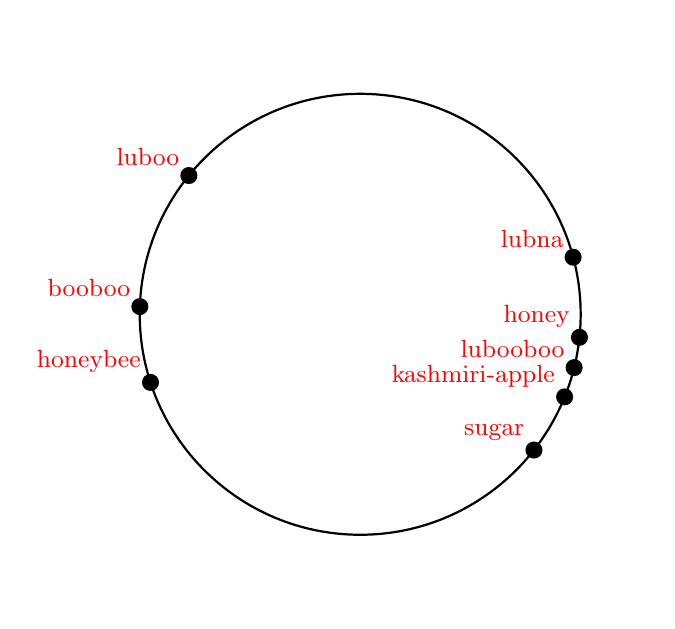
\begin{tikzpicture}[>=Stealth, line cap=round, line join=round, scale=2.8]
  \pgfextra{\path[use as bounding box] (-1.3,-1.3) rectangle (1.3,1.3);}
  \def\R{1.0}
  \draw[thick] (0,0) circle (\R);

  % Angles array
  \def\angles#1{\ifcase#1 15\or 141\or 178\or 198\or 322\or 338\or 346\or 354\fi}

  % Labels array
  \def\labels#1{\ifcase#1 lubna\or luboo\or booboo\or honeybee\or sugar\or kashmiri-apple\or lubooboo\or honey\fi}

  \foreach \i in {0,...,7}{
    \pgfmathsetmacro{\ang}{\angles{\i}}
    \fill[Oc] (\ang:\R) circle (1.1pt);
    \node[red, font=\small, anchor=south east] at (\ang:\R) {\labels{\i}};
  }

\end{tikzpicture}
\end{document}
